\documentclass[12pt]{book}
\usepackage[margin=.85in]{geometry} % for MARGIN
\usepackage[many]{tcolorbox}    	% for COLORED BOXES (tikz and xcolor included)


\usepackage{multicol}   
\usepackage{enumerate}
\usepackage[shortlabels]{enumitem}
\usepackage{varwidth}
\usepackage{tasks}
\usepackage[export]{adjustbox}

\usepackage{titleps}
\usepackage{setspace}               % for LINE SPACING
\usepackage[⟨options⟩]{fancyhdr}
\usepackage{enumitem}
\setlist{nosep}
\usepackage{tikz}
\usepackage{pgfplots}
\pgfplotsset{compat=1.5.1}
\usetikzlibrary{datavisualization}
\usetikzlibrary{datavisualization.formats.functions}

\newcommand{\D}{\displaystyle}


\setlength\parindent{0pt}   % killing indentation for all the text
\setstretch{1.3}            % setting line spacing to 1.3
\setlength\columnsep{0.25in} % setting length of column separator
\pagestyle{fancy}           % setting pagestyle to be headings

\usepackage[]{titlesec}

\fancyhead[L]{Math V04 - College Algebra}
\fancyhead[R]{Christina Papazacharioudakis}

\tcbset{
    sharp corners,
    colback = white,
    before skip = 0.2cm,    % add extra space before the box
    after skip = 0.5cm      % add extra space after the box
}                           % setting global options for tcolorbox

    \newtcolorbox{boxR}{
    fontupper = \color{black}, % font color
    boxrule = 1.5pt,
    colframe = black,
    rounded corners,
    arc = 5pt   % corners roundness
}

\definecolor{ballblue}{rgb}{0.13, 0.67, 0.8}

\begin{document}

\textbf{{\Large 2.4 Complex Numbers}}
\vspace{5mm}


{\large \textbf{Expressing Square Roots of Negative Numbers as Multiples of $i$}}
\vspace{3mm}

We know how to take the square root of any positive number. For example, $$ \sqrt{16} = 4$$

In a similar way, we can find the square root of any negative number and we call it an imaginary number.


\begin{boxR}
    The iaginary numer $i$ is defined to be the square root of $-1$.
    $$ \sqrt{-1}= i$$

Squaring both sides also gives us that $i^2 = -1$
\end{boxR}

This allows us to write the square root of any negative number using $i$. Let's consider the square root of $-49$:

\vspace{25mm}

Adding a real number and an imaginary number gives us complex numbers.
\vspace{3mm}

\begin{boxR}
\textbf{Imaginary and Complex Numbers}
    \vspace{1mm}
    \hline
    \vspace{2mm}
    A \textbf{complex number} is a number of the form $a + bi$ where: 
   \begin{itemize}
        \item $a$ is the real part of the complete number.
        \item $bi$ is the imaginary part of a complex number. 
    \end{itemize}
    \vspace{1mm}
    If $b=0$, then $a+bi$ is a real number. If $a=0$ and $b \neq 0$, the complex number is called a pure imaginary number. 
\end{boxR}

\newpage
\underline{\textbf{Example 1 - Expressing an Imaginary Number in Standard Form}}
Express the following numbers in standard form. 

\begin{enumerate}[(a)]
    \item $\sqrt{-9}$ 
    \vspace{30mm}
    \item $\sqrt{-24}$
     \vspace{30mm}
\end{enumerate}

\begin{boxR}
    \textbf{How To}
      \vspace{1mm}
    \hline
    \vspace{2mm}
    \textbf{Given an imaginary number, express it in the standard form of a complex number}
    \begin{enumerate}
        \item Write $\sqrt{-a}$ as $\sqrt{a}\sqrt{-1}$.
        \item Express $\sqrt{-1}$ as $i$.
        \item Write $\sqrt{a} \cdot i$ in simplest form.
    \end{enumerate}
\end{boxR}
\vspace{3mm}
{\large \textbf{Plotting a Complex Number on the Complex Plane}}
\vspace{3mm}

To graph a complex number, we use the \textbf{complex plane}. This is a coordinate system in which the horizontal axis represents the real component and the vertical axis represents the imaginary component.
Complex numbers $a+bi$ are expressed as the ordered pair $(a,b)$.

\newpage
\begin{boxR}
    \textbf{Complex Plane}
    \vspace{1mm}
    \hline
    \vspace{2mm}
    In the complex plane, the horizontal axis is the real axis, and the vertical axis is the imaginary axis, as shown below.
    
   \centerline{ 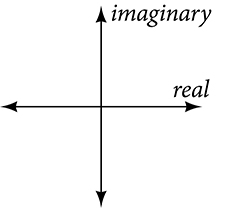
\includegraphics[height=40mm, width=40mm]{2.4-ComplexPlane.jpeg}}
\end{boxR}

\underline{\textbf{Example 2 - Plotting a Complex Number on the Complex Plane}}

Plot the complex numbers $3-4i$ and $-4-i$ on the complex plane. 

\begin{center}

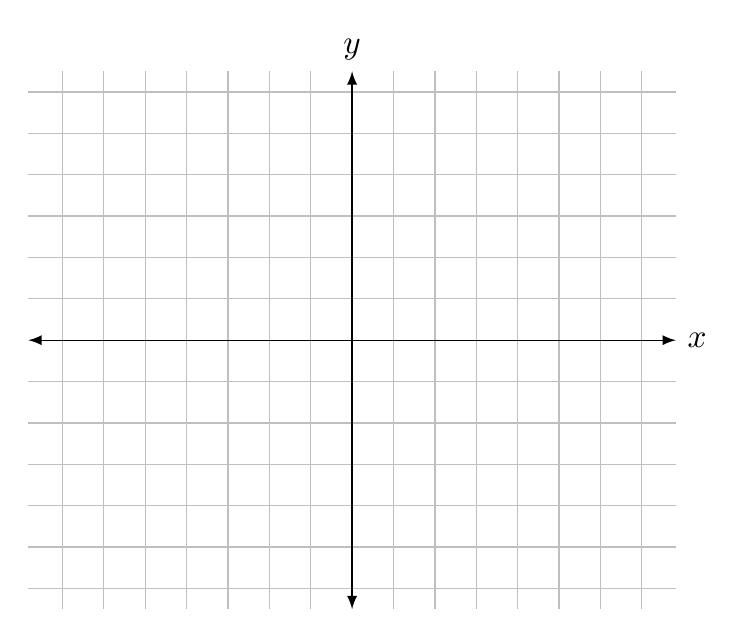
\begin{tikzpicture}[scale=1.2, transform shape]
\begin{axis}[
    ymin=-6.5,
    ymax=6.5,
    xmin=-6.5,
    xmax=6.5,
    axis on top=true,
    axis x line=middle,
    axis y line=middle,
    axis line style={latex-latex},
    xlabel=$x$,
    ylabel=$y$,
    xticklabels=\empty,
    yticklabels=\empty,
    xtick distance=1,
    ytick distance=1,
    xmajorgrids=true,
    ymajorgrids=true,
    axis equal = true, 
    every axis x label/.style={at={(ticklabel* cs:1.0)}, anchor=west,},
    every axis y label/.style={at={(ticklabel* cs:1.0)}, anchor=south,}
]
    \pgfplotsset{ticks=none}
\end{axis}
\end{tikzpicture}
\end{center}
\vspace{3mm}
{\large \textbf{Adding and Subtracting}}
\vspace{3mm}

Just as adding and subtracting real numbers, we can add and subtract complex numbers. 
\begin{boxR}
    \textbf{Complex Numbers: Addition and Subtraction}
    \vspace{1mm}
    \hline
    \vspace{2mm}
    Adding complex numbers: $$ (a+bi) + (c+di) = (a+c) + (b+d)i$$

    Subtracting complex numbers: $$ (a+bi) - (c+di) = (a-c) + (b-d)i$$
\end{boxR}
\newpage
\underline{\textbf{Example 3 - Adding and Subtracting Complex Numbers}}

Add or subtract as indicated.
\begin{enumerate}[(a)]
    \item $(3-4i) + (2+5i)$
    \vspace{35mm}
    \item $(-5+7i) - (-11 + 2i)$
    \vspace{35mm}
\end{enumerate}


\begin{boxR}
    \textbf{How To}
    \vspace{1mm}
    \hline
    \vspace{2mm}
    \textbf{Given two complex numbers, find the sum or difference.}
    \begin{enumerate}
        \item Identify the real and imaginary parts of each number.
        \item Add or subtract the real parts.
        \item Add or subtract the imaginary parts.
    \end{enumerate}
\end{boxR}

{\large \textbf{Multiplying Complex Numbers}}
\vspace{3mm}

Multiplying complex numbers is much like multiplying binomials. The major difference is that we work with the real and imaginary parts separately.
\vspace{3mm}

\textbf{Multiplying a Complex Number by a Real Number}

Lets begin by multiplying a complex number by a real number. We 
distribute the real number, as we would with a binomial. Consider, for example,  $3(6+2i)$:

\newpage

\begin{boxR}
    \textbf{How To}
    \vspace{1mm}
    \hline
    \vspace{2mm}
\textbf{Given a complex number and a real number, multiply to find the product.}
\begin{enumerate}
    \item Use the distributive property.
    \item Simplify.
\end{enumerate}
\end{boxR}

\underline{\textbf{Example 4 - Multiplying a Complex Number by a Real Number}}

Find the products $4(2+5i)$ and $\frac{1}{2}(5-2i)$.

\vspace{30mm}

\textbf{Multiplying Complex Numbers Together}

Our goal now is to multiply two complex numbers: $(a+bi)(c+di)$
\vspace{1mm}

Because we are dealing with binomials, we will use the FOIL method to multiply complex numbers together. As a reminder, FOIL stands for: 
\vspace{20mm}

\underline{\textbf{Example 5 - Multiplying a Complex Number by a Complex Number}}

Multiply: $(4+3i)(2-5i)$
\vspace{55mm}
\begin{boxR}
    \textbf{How To}
    \vspace{1mm}
    \hline
    \vspace{2mm}
\textbf{Given two complex numbers, multiply to find the product.}
\begin{enumerate}
    \item  Use the distributive property or the FOIL method.
    \item Remember that $i^2 = -1$
    \item Group together the real terms and the imaginary terms.
\end{enumerate}
\end{boxR}
\newpage
{\large \textbf{Dividing Complex Numbers}}
\vspace{3mm}

Dividing two complex numbers is more complicated than adding, subtracting, or multiplying. This is because dividing complex numbers does not immediately give us a complex number in standard form. Our goal now is figure out how we can rewrite the fraction below in standard form:$$ \frac{a+bi}{c+di}$$
We get the standard form of a complex number when the denominator is only a real number. So, how do we get there? We multiply the numerator and denominator by the \textbf{complex conjugate of the denominator}. This gives us a denominator of only real numbers. 
\vspace{3mm}
\begin{boxR}
     \textbf{The Complex Conjugate}
    \vspace{1mm}
    \hline
    \vspace{2mm}
    The \textbf{complex conjugate} of a complex number $a+bi$ is $a-bi$.
  It is found by changing the sign of the imaginary part of the complex number. The real part of the number is left unchanged.
\begin{itemize}
    \item When a complex number is multiplied by its complex conjugate, the result is a real number.
    \item When a complex number is added to its complex conjugate, the result is a real number.
\end{itemize}
\end{boxR}
\vspace{3mm}
\underline{\textbf{Example 6 - Finding Complex Conjugates}}

Find the complex conjugate $2 + 5i$. Then look at the product of the conjugate pairs. 



\newpage
\vspace{3mm}
\begin{boxR}
     \textbf{How To}
    \vspace{1mm}
    \hline
    \vspace{2mm}
 \textbf{ Given two complex numbers, divide one by the other.}
\begin{enumerate}
    \item Write the division problem as a fraction.
    \item Determine the complex conjugate of the denominator.
    \item Multiply the numerator and denominator of the fraction by the complex conjugate of the denominator.
    \item Simplify.
\end{enumerate}
\end{boxR}
\vspace{3mm}
\underline{\textbf{Example 7 - Dividing Complex Numbers}}

Divide: $(2+5i)$ by $(4-i)$

\vspace{50mm}

{\large \textbf{Simplifying Powers of $i$}}

Powers of $i$ have some repeating patterns. Let's take a look at what happens when we raise $i$ to increasing powers. 
\begin{multicols}{3}
  $i^1 = \\
    i^2 = \\
    i^3 = \\
    i^4 = \\
    i^5 = \\
    i^6 = \\
    i^7 = \\
    i^8 = \\
    i^9 = \\
    i^{10} = \\
    i^{11} = \\ 
    i^{12} = 
$
\end{multicols}

\vspace{3mm}
We can see that the following cycle repeats every four powers: 

\vspace{3mm}

To simplify powers of $i$, we can see simplify the problem by factoring out as many factors of $i^4$ as possible. Lets take a look!
\newpage

\underline{\textbf{Example 8 - Simplifying Powers of $i$}}

Evaluate: $i^{35}$.


\end{document}





